\documentclass{article}
\usepackage{fullpage}
\usepackage{indentfirst}
\usepackage{amsmath}
\usepackage{amsfonts}
\usepackage{pifont}
\usepackage{tipa}
\usepackage{tikz}
\usepackage{tikz-qtree}
\usetikzlibrary{matrix}
\usepackage{gb4e}
\noautomath
\title{Narrowing down a Topic}
\author{Chris Oakden}
\begin{document}
\maketitle
\section{Tonal Representation in Yip 2002 (ch 3)}
Yip (2002) outlines the following design desiderata for a feature system of tone:
\begin{exe}
\ex
\begin{xlist}
	\ex Characterize all and only the numbers of level tone contrasts (at least four, probably five)
	\ex Characterize contour tones, and their relationship to level tones (rising, falling, convex, concave, sometimes the result of combining two or more levels)
	\ex Characterize all and only the numbers of contour tone contrasts (two, possibly three of a given shape)
	\ex Allow for simple statements of common tonal alternations (assimilation, dissimilation, contour formation and simplification, downstep) 
	\ex Allow for simple statements about tonal markedness
	\ex Characterize the relationship between tonal and non-tonal features, particularly laryngeal features, both synchronically and historically
\end{xlist}
\end{exe}
After some discussion of a number of competing models, Yip identifies the model in Bao (1999) as the tonal model with the widest empirical coverage, and therefore the most desirable. In this model, tonal features ``are dominated by a node of their own, called Contour, which is a sister to the Register feature, and where both are dominated by a Tonal Node" (53).
\begin{exe}
\ex
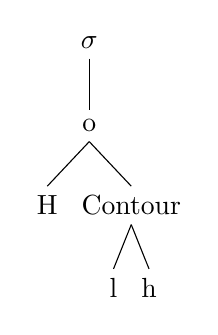
\begin{tikzpicture}[baseline = (current bounding box.north)]
\Tree [.$\sigma$ [.o [.H ] [.Contour [.l ] [.h ]]]] 
\end{tikzpicture}
\end{exe}
This representation predicts a number of observed spreading patterns which other models do not, accomodating register spread (in Chaozhou), contour spreading (in Zhenhai), and whole tone spreading/copying (in Danyang) equally well. An example of register spreading in Ewe (Clements 1978, Odden 1995) is given in (\ref{Ewe}):
\begin{exe}
\ex \label{Ewe}
\begin{tikzpicture}[baseline=(m-1-1.base)]
\matrix (m) [matrix of nodes, row sep = .75em] {
$w$ & $v$   \\
$w'$ & $v'$  \\
};
\end{tikzpicture}
\end{exe}
Registers can also account for tone systems with more than one of the same contrastive contour, for example a language which has a high falling and low falling tone. Yip uses the fact that contours in many Chinese dialects usually occupy only the upper or lower half of the pitch range to argue for this representation.
\begin{exe}
\ex
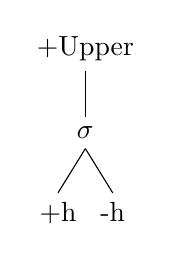
\begin{tikzpicture}[baseline=(current bounding box.north)]
\Tree [.+Upper [. $\sigma$ [.+h ] [.-h ]]]
\end{tikzpicture}
~ 53 High-falling
\hspace{2cm}
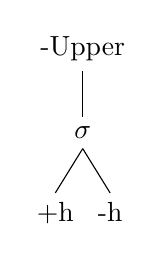
\begin{tikzpicture}[baseline=(current bounding box.north)]
\Tree [.-Upper [. $\sigma$ [.+h ] [.-h ]]]
\end{tikzpicture}
~ 13 Low-falling
\end{exe}
\par With respect to the structure of contours, Yip presents evidence of contours both as sequences of level tones and as units, but does not provide a definitive answer as to their true composition. If contour tones are decomposable into level units, the expectation is that they comprise only the level tones available in the language. One counterexample to this claim is Mandarin Chinese, which has a [35] rising tone (MH), but no mid, level tone (33).
\par Reading through this chapter, I have thought of some basic questions that might lead me closer to narrowing down a topic. Here are some of them.
\begin{itemize}
	\item Assuming a tonal model like Bao (1999), spreading patterns at each of three hierarchical levels (Tonal Node, Register, Contour) can be formalized. What about dissimilatory patterns (which comprise a large portion of tone sandhi)? Chen (2000) claims that register dissimilation is basically non-existent in Chinese tone sandhi; how can we account for this typological gap?
	\item A full model with a specified register basically prevents contours which use more than the upper or lower half of the pitch range, since each tonal node dominates a register node specified as either [+U] or [-U]. This seems to contradict a number of attested contour tones, like Mandarin 4th tone (falling), which often takes the Chao numbers [51]. How can these be represented?
	\item Yip says that derived contours (often observed in African tone languages) are ``clusters of two tones formed by reassociation of stranded tones," and that these tones often span over the entire pitch range, ``as one might expect if they are formed by the concatenation of the H and L of a two-tone system" (49). This doesn't make sense; earlier, Yip says that units like H and L are actually just a shorthand for matrices of register and contour features ([+U, +h], [-U, -h], etc.). If this is the case, what are stranded tones' true representation? Are they unspecified for register? And if we allow underspecification, don't we also expect stranded tones which carry no contour specification (i.e. just +Upper/-Upper register)?
	\item What exactly is the TBU in this model? Yip describes contours as comprising ``two (or more) tones associated with one syllable (or perhaps vowel or  mora)" (48). In Bao's model, tones only associate to the syllable transitively through the Tonal Node, with vowels and morae nowhere in sight. What type of predictions does this make, especially in terms of tone-stress/prominence interaction (among others)?
	\item The adopted model accounts for observed patterns, but does it rule out unattested ones? The fourth criterion in selecting a tonal model states that the representation should allow for simple statements of common tonal alternations, however this statement doesn't seem to require any restrictive power from the model. 
	\item Although not explicitly stated, locality seems to be a very basic restriction on sandhi and tonal processes in general; spreading and delinking happens on adjacent tones and syllables. Does the current model formalize that in any way? Is there a way to formalize this restriction?
\end{itemize}
\section{Sandhi Generalizations as Melody-Local Grammars?}
Tone sandhi in Chinese dialects is local in a broad sense; sandhi patterns do not occur in which tones on disjoint syllables vary, leaving intervening syllables unaltered. However, the nature of this locality must be defined. Sandhi alternations from two dialects exhibit the significance of the locality question.
Recall disyllabic sandhi in Tianjin.
\begin{exe}
\ex
\label{x:Tianjin1}
\begin{tabular}[t]{ccc}
 Input && Output \\
 \hline
LL & $\rightarrow$ & RL \\
RR & $\rightarrow$ & HR \\
FF & $\rightarrow$ & LF \\
FL & $\rightarrow$ & HL \\
\end{tabular}
\end{exe}
The four patterns described above are dissimilatory in nature, and can be conceptualized as OCP effects. But what is the locus of the OCP restrictions here? The first three patterns are syllable-level dissimilation alternations, that is, the prohibited sequences in question are syllables with the same tonal specification (low tone, rising tone, falling tone). The fourth pattern suggests an OCP effect crucially on the melodic tier; understanding falling tone as HL, the ill-formed structure is a sequence of two adjacent L tones across a syllable boundary (HL.LL). 
Additionally, the first three patterns cannot be described unambiguously as derivable from melodic-tier OCP. The RR (or $\mathtt{cntr}$(RR) = LHLH) and FF (or $\mathtt{cntr}$(FF) = HLHL) sequences do not violate OCP in their melodies (though the restrictions can be represented straightforwardly as strings of morae). Their representation as [LH] and [HL] respectively is felicitous, however, as alternating surface forms appear to be the result of contour simplification, specifically deletion of the rightmost association on the initial syllable (LH $\rightarrow$ H, HL $\rightarrow$ L).
Understanding these patterns in terms of melody-local grammars does not clarify the locality issue. String and melody restrictions for these sandhi patterns are as follows:
\begin{exe}
\ex
$\mathcal{S}_{TJ}$ = \{LLLL, LHLH, HLHL, HLLL\} \\
$\mathcal{M}_{TJ}$ = \{L, LHLH, HLHL, HL\}
\end{exe}
Evaluating the $\mathtt{mldy}(w)$ function on the string [LLLL] without reference to syllable boundaries yields [L], and [HL] on the string [HLLL]. This predicts a number of well-formed strings (like single L- and F-toned syllables) in the language to be ungrammatical. 
\begin{exe}
\ex
\begin{tabular}[t]{cllcc}
\hline
& $w$ & $\mathtt{mldy}(w)$ & $\mathcal{S}_{TJ}$ & $\mathcal{M}_{TJ}$ \\
\hline
a. & LL & L & $\checkmark$ & \ding{55} \\
b. & HL & HL & $\checkmark$ & \ding{55} \\
\hline
\end{tabular}
\end{exe}
Without reference to syllable boundaries, the alternation cannot be captured. Specifically, the melodic constraints are sensitive to syllable boundaries, and the evaluation of $\mathtt{mldy}(w)$ collapses these. 

Similar generalizations are true for tone sandhi in the Nanjing dialect. Recall the basic generalizations.
\begin{exe}
\ex
\begin{tabular}[t]{lcl}
 Input && Output \\
 \hline
FF & $\rightarrow$ & HF \\
LL & $\rightarrow$ & RL \\
LH & $\rightarrow$ & RH \\
LF & $\rightarrow$ & RF \\
RHq& $\rightarrow$ & LHq \\
HHq& $\rightarrow$ & FHq \\
\end{tabular}
\end{exe}
Again, both syllable-level and melodic-level dissimilatory patterns are apparent (as well as assimilatory alternations). String and melody restrictions are presented below.
\begin{exe}
\ex
$\mathcal{S}_{NJ}$ = \{HLHL, LLLL, LLHH, LLHL, LHH, HHH\} \\
$\mathcal{M}_{NJ}$ = \{HLHL, L, LH, LHL, H\}
\end{exe}
The same confounds observed in the Tianjin data emerge in the melody-local characterizations of Nanjing tone sandhi. 
\begin{exe}
\ex
\begin{tabular}[t]{cllcc}
\hline
& $w$ & $\mathtt{mldy}(w)$ & $\mathcal{S}_{NJ}$ & $\mathcal{M}_{NJ}$ \\
\hline
a. & LL & L & $\checkmark$ & \ding{55} \\
b. & LH & LH & $\checkmark$ & \ding{55} \\
c. & H & H & $\checkmark$ & \ding{55} \\
d. & LHLH & LHLH & $\checkmark$ & \ding{55} \\
\hline
\end{tabular}
\end{exe}
Grammatical strings are predicted to be ungrammatical by the set of ungrammatical melodies $\mathcal{M}_{NJ}$. \par
It would appear that melody-locality is perhaps not the right way to approach these problems, since melody-local restrictions are used to capture long-distance tonal patterns. But, there is an intuition that there is more than one \emph{type} of locality at play in tone sandhi. \par
In a melody-local model, melodic-tier restrictions are \emph{derived} from string representations via the $\mathtt{mldy}(w)$ function to capture non-local patterns. The function's output is a condensed form of the string representation that characterizes ill-formed structures. Here are some questions about this function as it applies to the current topic:
\begin{itemize}
	\item Would a similar approach prove fruitful in characterizing tone sandhi using Bao's model? 
	\item Can the hierarchical relationship between syllable/TBU, Tonal Node, Register Node, and Contour Node be extracted from string representation via some set of functions? 
	\item Would this require three (or more) sets of constraints that target each level? And if so, could this provide the reference to syllable boundaries that is needed to disambiguate grammatical and ungrammatical structures in specific languages?
	\item Or do we need to enrich the representation to include syllable boundaries? How (and where) are these represented and are there any undesirable consequences from this representation?
\end{itemize}
\end{document}